\chapter{Information to subjects}
\section{Project title: Can mindfulness alter sensitivity pain?} 
We would like to enquire if you are interested in participating in a 8th semester project of Biomedical Engineering and Informatics which is to be performed at Aalborg University.
Before you decide to participate in the project, it is important that you fully understand the procedures of the experiment. Therefore, we ask you kindly to read this information carefully.
Participation in the project is voluntary. You can at any time and without stating a reason withdraw your consent.

\section{Purpose of the experiment}
Approximately 375 million people suffer from chronic neck pain. The current treatment methods only provide relieve of pain but there is no cure.  The primary treatment for those patients is medication. However, medication has side effects such as abuse or organ damage. Alternative methods exist like mindfulness meditation. Previous studies have investigated the usefulness of mindfulness meditation for people suffering from chronic pain showing promising results in pain relief. For this reason, the present study want to address if ‘Short-term mindfulness meditation practice increases the pressure pain threshold and the pressure pain tolerance’.

\section{Who can participate?}
You can participate in the trial if you fulfill the specific inclusion and exclusion criteria formed for this experiment. 

Inclusion criteria:
\begin{itemize}
	\item Healthy
	\vspace{-.3cm}
	\item Age between 20 and 30 years
	\vspace{-.3cm}
	\item Normal BMI (F: 19-24 M: 20-25)
	\vspace{-.3cm}
	\item Must have time to meditate for 5 days, 30 minutes per day.
\end{itemize}

Exclusion criteria:
\begin{itemize}
	\item Ongoing meditation practice 
	\vspace{-.3cm}
	\item Acute or chronic pain
	\vspace{-.3cm}
	\item Pregnancy 
	\vspace{-.3cm}
	\item Neurological, musculoskeletal or mental illness
	\vspace{-.3cm}
	\item Signs or symptoms of any serious systemic diseases 
	\vspace{-.3cm}
	\item Psychiatric, analgesic or other medications that might influence their response to pain 
		\vspace{-.3cm}
	\item Abusive drug or alcohol use
	\vspace{-.3cm}
	\item Lack of ability to cooperate
\end{itemize}

Further, you must be able to speak and understand English or Danish.
 
\section{Experiment}
The experiment consist of two measurement sessions, each lasting about 30 minutes. The sessions will be conducted with intervals of one week between them. At the measurement  session, we will apply pressure in both sides of the upper trapezius, as illustrated in \figref{fig:trapezius}, with and algometer in order to determine the pressure pain threshold and the pressure pain tolerance. 

\begin{figure}[H]
	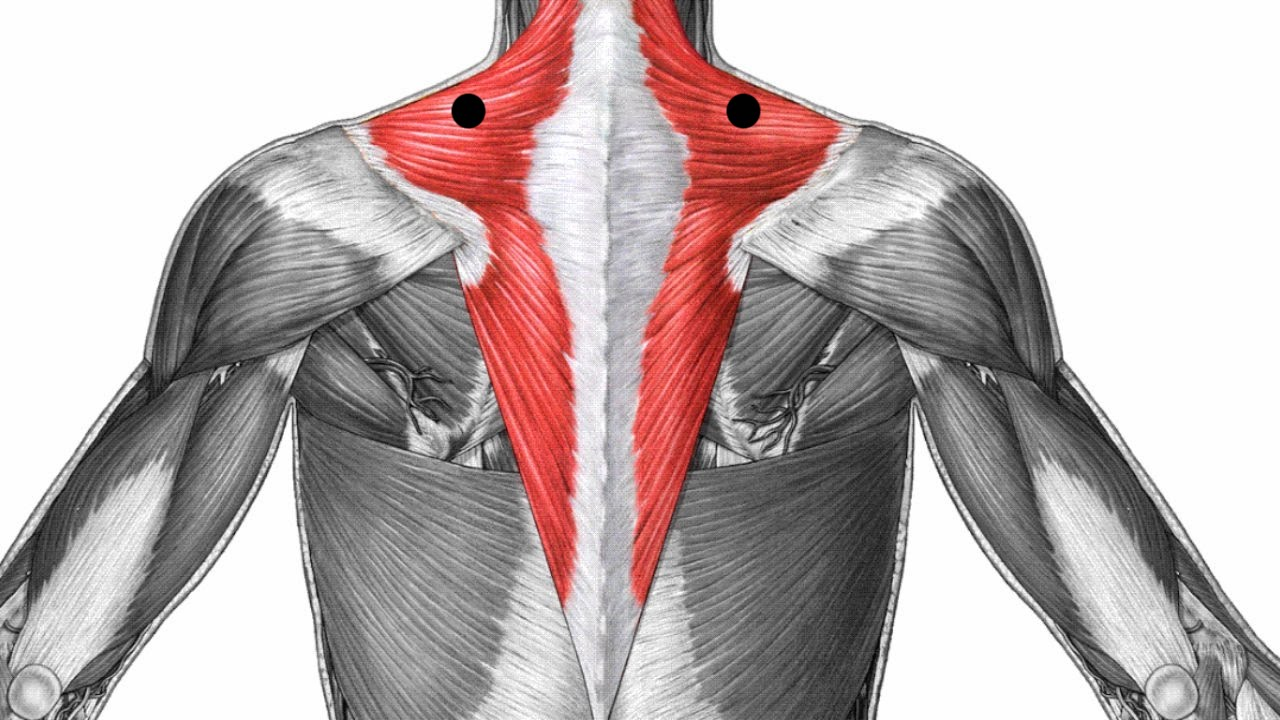
\includegraphics[width=0.5\textwidth]{figures/trapezius.jpg}
	\caption{Measurement points on the upper trapezius}
	\label{fig:trapezius} 
\end{figure}

The subject are divided into two groups - a treatment group and a control group. This is done randomly.

Between the first measurement session and the second measurement the treatment group will practice guided mindfulness meditation for 5 consecutive days, each session lasting about 20 minutes. The control group will continue their normal routine between the two measurements.


\section{Risk and side effects}
The experimental methods used in this study are well tested and have been used in several studies . No side effects have been reported from these studies.


\section{Benefits of the experiment}
There will be no immediate personal gain associated with your participation in the trial. However, we expect that the results of the study may contribute to knowledge within alternative methods, in this case, mindfulness meditation to relieve pain in people with chronic pain. Furthermore you will get an insight in mindfulness meditation and the benefits from practicing it.

\section{Exclusion from and suspension of experiment}
If you are not suitable for continuing in the experiment, your participation can be terminated at any time.
None of the researchers have financial interest in the study.

Contact information
18gr8405@hst.aau.dk
Phone: XXXXXXXX
